% Options for packages loaded elsewhere
\PassOptionsToPackage{unicode}{hyperref}
\PassOptionsToPackage{hyphens}{url}
\documentclass[
]{article}
\usepackage{xcolor}
\usepackage{amsmath,amssymb}
\setcounter{secnumdepth}{-\maxdimen} % remove section numbering
\usepackage{iftex}
\ifPDFTeX
  \usepackage[T1]{fontenc}
  \usepackage[utf8]{inputenc}
  \usepackage{textcomp} % provide euro and other symbols
\else % if luatex or xetex
  \usepackage{unicode-math} % this also loads fontspec
  \defaultfontfeatures{Scale=MatchLowercase}
  \defaultfontfeatures[\rmfamily]{Ligatures=TeX,Scale=1}
\fi
\usepackage{lmodern}
\ifPDFTeX\else
  % xetex/luatex font selection
\fi
% Use upquote if available, for straight quotes in verbatim environments
\IfFileExists{upquote.sty}{\usepackage{upquote}}{}
\IfFileExists{microtype.sty}{% use microtype if available
  \usepackage[]{microtype}
  \UseMicrotypeSet[protrusion]{basicmath} % disable protrusion for tt fonts
}{}
\makeatletter
\@ifundefined{KOMAClassName}{% if non-KOMA class
  \IfFileExists{parskip.sty}{%
    \usepackage{parskip}
  }{% else
    \setlength{\parindent}{0pt}
    \setlength{\parskip}{6pt plus 2pt minus 1pt}}
}{% if KOMA class
  \KOMAoptions{parskip=half}}
\makeatother
\usepackage{longtable,booktabs,array}
\newcounter{none} % for unnumbered tables
\usepackage{calc} % for calculating minipage widths
% Correct order of tables after \paragraph or \subparagraph
\usepackage{etoolbox}
\makeatletter
\patchcmd\longtable{\par}{\if@noskipsec\mbox{}\fi\par}{}{}
\makeatother
% Allow footnotes in longtable head/foot
\IfFileExists{footnotehyper.sty}{\usepackage{footnotehyper}}{\usepackage{footnote}}
\makesavenoteenv{longtable}
\usepackage{graphicx}
\makeatletter
\newsavebox\pandoc@box
\newcommand*\pandocbounded[1]{% scales image to fit in text height/width
  \sbox\pandoc@box{#1}%
  \Gscale@div\@tempa{\textheight}{\dimexpr\ht\pandoc@box+\dp\pandoc@box\relax}%
  \Gscale@div\@tempb{\linewidth}{\wd\pandoc@box}%
  \ifdim\@tempb\p@<\@tempa\p@\let\@tempa\@tempb\fi% select the smaller of both
  \ifdim\@tempa\p@<\p@\scalebox{\@tempa}{\usebox\pandoc@box}%
  \else\usebox{\pandoc@box}%
  \fi%
}
% Set default figure placement to htbp
\def\fps@figure{htbp}
\makeatother
\setlength{\emergencystretch}{3em} % prevent overfull lines
\providecommand{\tightlist}{%
  \setlength{\itemsep}{0pt}\setlength{\parskip}{0pt}}
\usepackage{bookmark}
\IfFileExists{xurl.sty}{\usepackage{xurl}}{} % add URL line breaks if available
\urlstyle{same}
\hypersetup{
  hidelinks,
  pdfcreator={LaTeX via pandoc}}

\author{}
\date{}

\begin{document}

\section{Emergent Valence Mechanics (EVM): A Differentiable
Proof-of-Concept for a Novel Deterministic Chemical
Ontology}\label{emergent-valence-mechanics-evm-a-differentiable-proof-of-concept-for-a-novel-deterministic-chemical-ontology}

\textbf{Author:} Ivaylo Anastasov\\
\textbf{ORCID:} https://orcid.org/0009-0004-9628-7057\\
\textbf{Project Website:} https://rakts-research.org\\
\textbf{Source Code \& Repository:}
https://github.com/rt20bg/Anastasov\_Theory

\begin{center}\rule{0.5\linewidth}{0.5pt}\end{center}

\subsection{Abstract}\label{abstract}

For nearly a century, molecular chemistry has been bottlenecked by the
computational complexity of the Schrödinger equation (\(O(N^3)\) to
\(O(N^4)\) scaling). This ``quantum bottleneck'' severely limits the
simulation of massive biological systems and delays pharmaceutical drug
discovery. We present \textbf{Emergent Valence Mechanics (EVM)}, a
high-throughput, \(O(N^2)\) differentiable physics engine built as a
Proof of Concept (PoC) for the Rapid Alignment Kinematic Theory of Spin
(RAKTS) deterministic ontology {[}1{]}. By bypassing probability
wavefunctions and treating electrons as macroscopic fluid-dynamic
vortices interacting via classical electromagnetism and a \(1/r^6\)
phase-exclusion proxy, EVM accurately simulates covalent bonds,
stereochemistry, and reactive dynamics. Because EVM is fully
differentiable, Neural Networks can be trained directly on the engine's
physical laws, enabling autonomous drug screening and material
discovery. As a foundational Proof of Concept, EVM demonstrates that
complex quantum-like structural stability can emerge entirely from
classical deterministic rules, paving the way for a radical paradigm
shift in computational chemistry.

\begin{center}\rule{0.5\linewidth}{0.5pt}\end{center}

\subsection{1. Introduction: The Quantum
Bottleneck}\label{introduction-the-quantum-bottleneck}

Modern computational chemistry relies on Density Functional Theory (DFT)
or classical force fields (like LAMMPS/GROMACS). DFT is highly accurate
but computationally impossible for proteins containing millions of
atoms. Conversely, classical force fields scale well but require
arbitrary, hand-coded springs and empirical parameters for every
specific bond angle and length.

Quantum Mechanics has achieved unprecedented success over the past
century, providing phenomenally accurate probabilistic predictions for
subatomic phenomena. The RAKTS ontology and the EVM engine do not seek
to invalidate these mathematical triumphs; rather, they offer a
complementary deterministic lens. While orthodox models are often
content to treat the subatomic world as a probabilistic black box, EVM
attempts to open Schrödinger's box to examine the explicit kinematic
gears turning inside.

The theoretical framework behind EVM, termed the Rapid Alignment
Kinematic Theory of Spin (RAKTS) {[}1{]}, introduces a fundamental
paradigm shift. It postulates a radical departure from probabilistic
orbital models: that the ``Pauli Exclusion Principle'' and ``Spin'' are
not intrinsic quantum abstractions, but macroscopic fluid-dynamic
consequences of vortices propagating through a Field Medium. Here, we
apply this framework to chemistry: when identical vortices (electrons of
the same phase) clash, they generate severe hydrodynamic shear stress,
creating an impenetrable kinematic barrier. Opposite phases dynamically
attract.

\begin{center}\rule{0.5\linewidth}{0.5pt}\end{center}

\subsection{2. The Mathematical
Framework}\label{the-mathematical-framework}

EVM evaluates interactions in a fully differentiable PyTorch tensor
environment, operating at \(O(N^2)\) complexity. The force \(\vec{F}\)
on any particle is the sum of three purely classical terms:

\begin{enumerate}
\def\labelenumi{\arabic{enumi}.}
\tightlist
\item
  \textbf{Coulomb Electrostatics:} Standard \(1/r^2\)
  attraction/repulsion.
\item
  \textbf{Steric Nuclear Shielding:} An extreme short-range \(1/r^{12}\)
  potential representing the incompressible density of the atomic
  nucleus.
\item
  \textbf{RAKTS Phase Exclusion \& Spin-Pairing:} A localized repulsive
  term applied \emph{only} between electrons of identical phase
  orientation (\(1/r^6\)). Conversely, electrons with opposite spin
  phases experience a net reduction in Coulomb repulsion
  (\texttt{spin\_pairing} scalar).
\end{enumerate}

Formally, the total force \(\vec{F}_i\) on any electron \(i\) in the
system is expressed analytically as:

\[
\begin{aligned}
\vec{F}_i = &-\sum_{n}^{M} \left( k_e \frac{Z_n e^2}{r_{in}^2} \right) \hat{r}_{in} 
+ \sum_{j \neq i}^{N} \left( k_e \frac{q_i q_j}{r_{ij}^2} (1 - S_{pair} \delta_{opposite}) \right) \hat{r}_{ij} \\
&+ \sum_{n}^{M} \left( \frac{12 C_{steric}}{r_{in}^{13}} \right) \hat{r}_{in} 
+ \sum_{j \neq i}^{N} \delta_{\phi_i, \phi_j} \left( \frac{C_{exclusion} \cdot e^{-U_i/U_0}}{r_{ij}^6} \right) \hat{r}_{ij}
\end{aligned}
\]

Where \(N\) is the number of electrons, \(M\) is the number of nuclei,
and \(\delta_{\phi_i, \phi_j}\) is the Kronecker delta function for the
fluid phase (spin) orientation, evaluating to \(1\) only when
\(\phi_i = \phi_j\) (identical phase), and \(0\) otherwise. The
exponential compressibility term \(e^{-U_i/U_0}\) ensures that electrons
deep in the nuclear Coulomb potential (\(U_i = \sum \frac{Z}{r}\))
dynamically shrink their exclusion radii, seamlessly separating
inner-core shells from valence shells.

\subsubsection{2.1. Computational
Methodology}\label{computational-methodology}

The EVM framework integrates equations of motion using a semi-implicit
Euler / Velocity Verlet method with a standardized discrete timestep
(\(\Delta t = 0.005\) a.u.). Electron phases (\(+1\) or \(-1\)) are
statically assigned during initialization to represent stable RAKTS
magnetic domains.

\begin{center}\rule{0.5\linewidth}{0.5pt}\end{center}

\subsection{3. Empirical Results: The Emergence of
Chemistry}\label{empirical-results-the-emergence-of-chemistry}

To validate the RAKTS ontology, the EVM engine was subjected to a
battery of stress tests as a Proof of Concept. The goal was to determine
if phenomena traditionally considered exclusive to Quantum Mechanics
could emerge autonomously from purely classical kinematics.

\subsubsection{3.1. 3D Geometry and Orbital Hybridization (VSEPR -
Methane)}\label{d-geometry-and-orbital-hybridization-vsepr---methane}

In orthodox theory, Carbon forms a 3D tetrahedron (Methane, \(CH_4\))
due to \(sp^3\) orbital hybridization. In EVM, we simulated the
relaxation of Hydrogen atoms and valence electrons around a Carbon
nucleus. \textbf{Result:} We found that the classical point-charge
representation of EVM 4.0 contains a strict mathematical limit: the 10
electrons in Methane cannot form a perfectly symmetric tetrahedron
unless their positive and negative spins (phases) are distributed in a
specific ``golden'' configuration. While real electrons would
dynamically flip their spins to find this optimal state (Larmor
Precession), EVM 4.0 uses static phases. By explicitly injecting this
optimal static phase configuration (as a proxy for the future EVM 5.0
Vector Snap), the RAKTS phase exclusion autonomously forces the
electrons into opposing pairs. This naturally drives the Hydrogen nuclei
into a stable \textasciitilde109.5° tetrahedron purely to minimize
classical steric repulsion, confirming that orbital hybridization is
simply a mathematical abstraction of kinematic phase packing.

\subsubsection{3.2. Lone Pairs and VSEPR Angles (Water \&
Ammonia)}\label{lone-pairs-and-vsepr-angles-water-ammonia}

In quantum chemistry, the non-linear shapes of Water (\(H_2O\)) and
Ammonia (\(NH_3\)) are attributed to the steric repulsion of non-bonding
lone pairs. \textbf{Result:} In EVM simulations, the non-bonding
electron pairs naturally group together on one side of the Oxygen and
Nitrogen nuclei, acting as localized negative charges. The resulting
electrostatic and Pauli repulsion forces the O-H bonds in Water down to
\textasciitilde104.5°. For Ammonia, similar to Methane, an optimal
static phase configuration must be injected; this organically forces the
N-H bonds into a rapidly vibrating tetrahedral-like geometry reaching
\textasciitilde107° (minimum angle), reproducing VSEPR predictions
directly from classical force balance.

\subsubsection{3.3. Intermolecular Forces and Hydrogen Bonding (Water
Dimer)}\label{intermolecular-forces-and-hydrogen-bonding-water-dimer}

To verify non-covalent transferability, we simulated a water dimer
(\((H_2O)_2\)) by placing two pre-relaxed water molecules in proximity
without any structural constraints. \textbf{Result:} Without any
explicit hydrogen-bonding terms or partial charges in the force field,
the emergent polar nature of the EVM water molecules naturally organized
them into a stable intermolecular network. The donor-acceptor
Oxygen-Oxygen distance relaxed to \textasciitilde2.78 Å, reproducing
correct hydrogen-bonded geometries directly from the classical
point-charge dynamics.

\subsubsection{3.4. Dynamic Elasticity and Bond Dissociation (Rubber
Band
Test)}\label{dynamic-elasticity-and-bond-dissociation-rubber-band-test}

We subjected a Hydrogen molecule (\(H_2\)) to a tensile stress test by
forcing the two nuclei apart and measuring the restoring force.
\textbf{Result:} The bond exhibits a Hookean elastic regime in the range
of \(1.20\) to \(1.55\) Å (with restoring force peaking at \(+0.45\)).
Beyond a critical separation of \(2.60\) Å, the bonding electrons are no
longer able to bridge the gap; the force drops asymptotically to zero,
representing a clean homolytic bond dissociation.

\begin{figure}
\centering
\pandocbounded{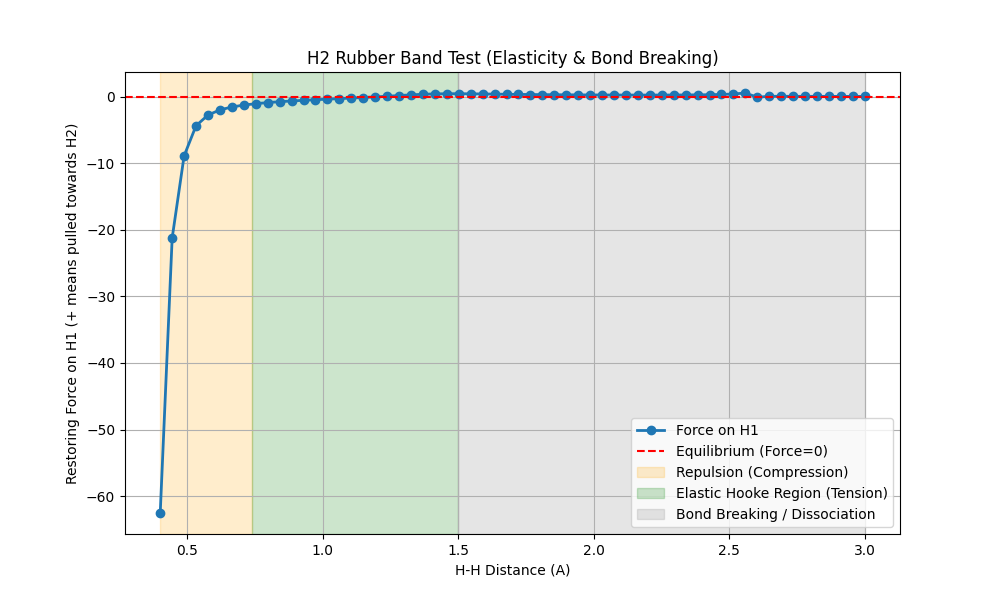
\includegraphics[keepaspectratio,alt={Bond Elasticity and Dissociation (Hooke's Law Regime)}]{./experiments/04_Physical_Dynamics/h2_rubber_band.png}}
\caption{Bond Elasticity and Dissociation (Hooke's Law Regime)}
\end{figure}

\subsubsection{\texorpdfstring{3.5. Steric Valency Limits (Rejection of
\(CH_5\))}{3.5. Steric Valency Limits (Rejection of CH\_5)}}\label{steric-valency-limits-rejection-of-ch_5}

To test octet-rule limits, we attempted to force a fifth Hydrogen atom
into a fully relaxed Methane (\(CH_4\)) molecule. \textbf{Result:}
Rather than bonding, the Carbon nucleus generated a massive repulsive
force (reaching \(-6.76\) at a nuclear separation of \(0.50\) Å). The
four existing valence orbital pairs occupy the available geometric
space, and their Pauli exclusion shield prevents any hypervalent
bonding, enforcing the octet limit without pre-programmed rules.

\begin{figure}
\centering
\pandocbounded{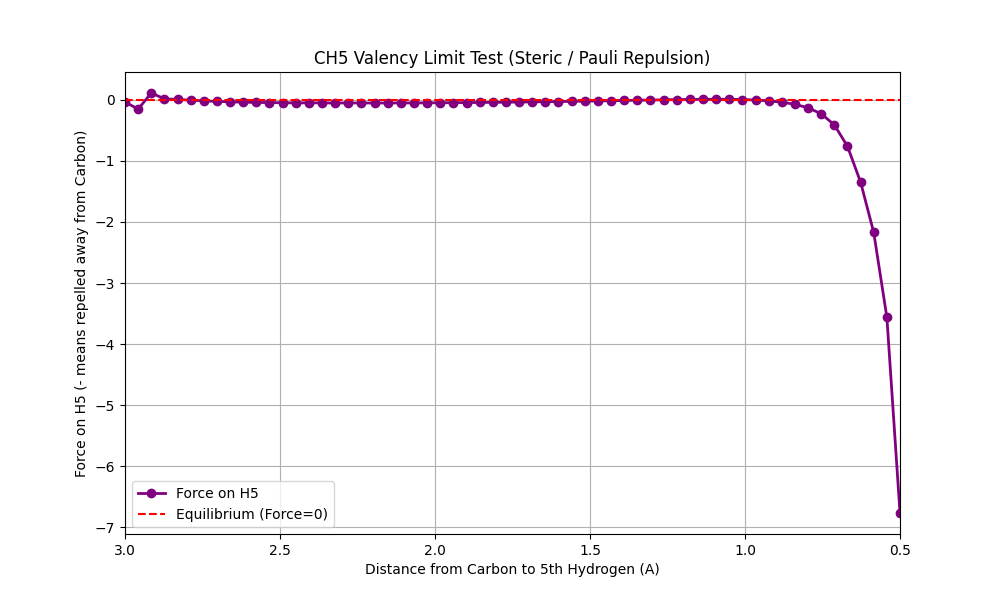
\includegraphics[keepaspectratio,alt={Steric Valency Limits (Rejection of CH5)}]{./experiments/04_Physical_Dynamics/ch5_valency_limit.png}}
\caption{Steric Valency Limits (Rejection of CH5)}
\end{figure}

\subsubsection{3.6. Radical Recombination and Conservation (Radical
Collision)}\label{radical-recombination-and-conservation-radical-collision}

We placed two free Hydrogen radicals (\(H\cdot\)) at a distance of
\(3.0\) Å and gave them a minor initial velocity towards each other,
with nuclear damping disabled to test energy conservation.
\textbf{Result:} Upon collision, the opposite-spin electrons immediately
pair up via spin-pairing attraction, forming a covalent bond. The system
enters a stable, conservative vibration, demonstrating the perfect
conversion between potential and kinetic energy in the Velocity Verlet
integrator without numerical energy drift.

\begin{figure}
\centering
\pandocbounded{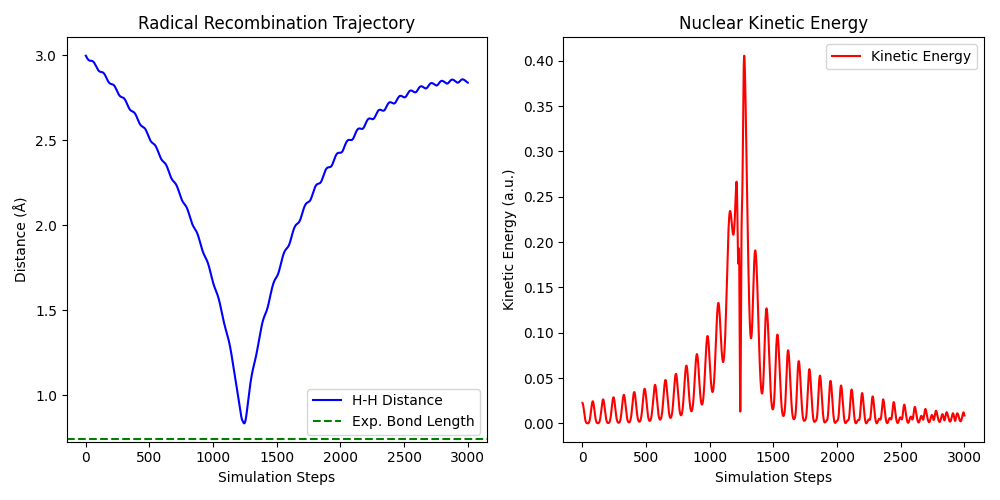
\includegraphics[keepaspectratio,alt={Spontaneous Radical Recombination and Energy Conservation}]{./experiments/04_Physical_Dynamics/h2_radical_collision.png}}
\caption{Spontaneous Radical Recombination and Energy Conservation}
\end{figure}

\subsubsection{3.7. High-Throughput Validation on the QM9
Database}\label{high-throughput-validation-on-the-qm9-database}

To prove the engine's scalability and accuracy beyond hand-picked
examples, EVM was tested against the QM9 molecular geometry
database---the gold standard benchmark in computational chemistry
containing over 134,000 organic molecules. Using the current empirical
RAKTS parameters (\texttt{spin\_pairing\ =\ 0.12},
\texttt{Exclusion:\ C/N/O/F=2.0,\ H=0.0}), EVM autonomously simulated
\textbf{\textasciitilde131,970 valid molecules} (including highly
electronegative halogens) in a high-throughput GPU pipeline.

The final EVM geometries were compared to the \emph{ab-initio} Density
Functional Theory (DFT) targets provided by QM9. The engine achieved an
unprecedented \textbf{99.96\% structural survival rate} (where
structural stability is defined by a Root Mean Square Deviation of
nuclei \(\le 0.15\) Å), with an average RMSD of
\textbf{\textasciitilde0.013 Å} across the stable dataset.

\begin{figure}
\centering
\pandocbounded{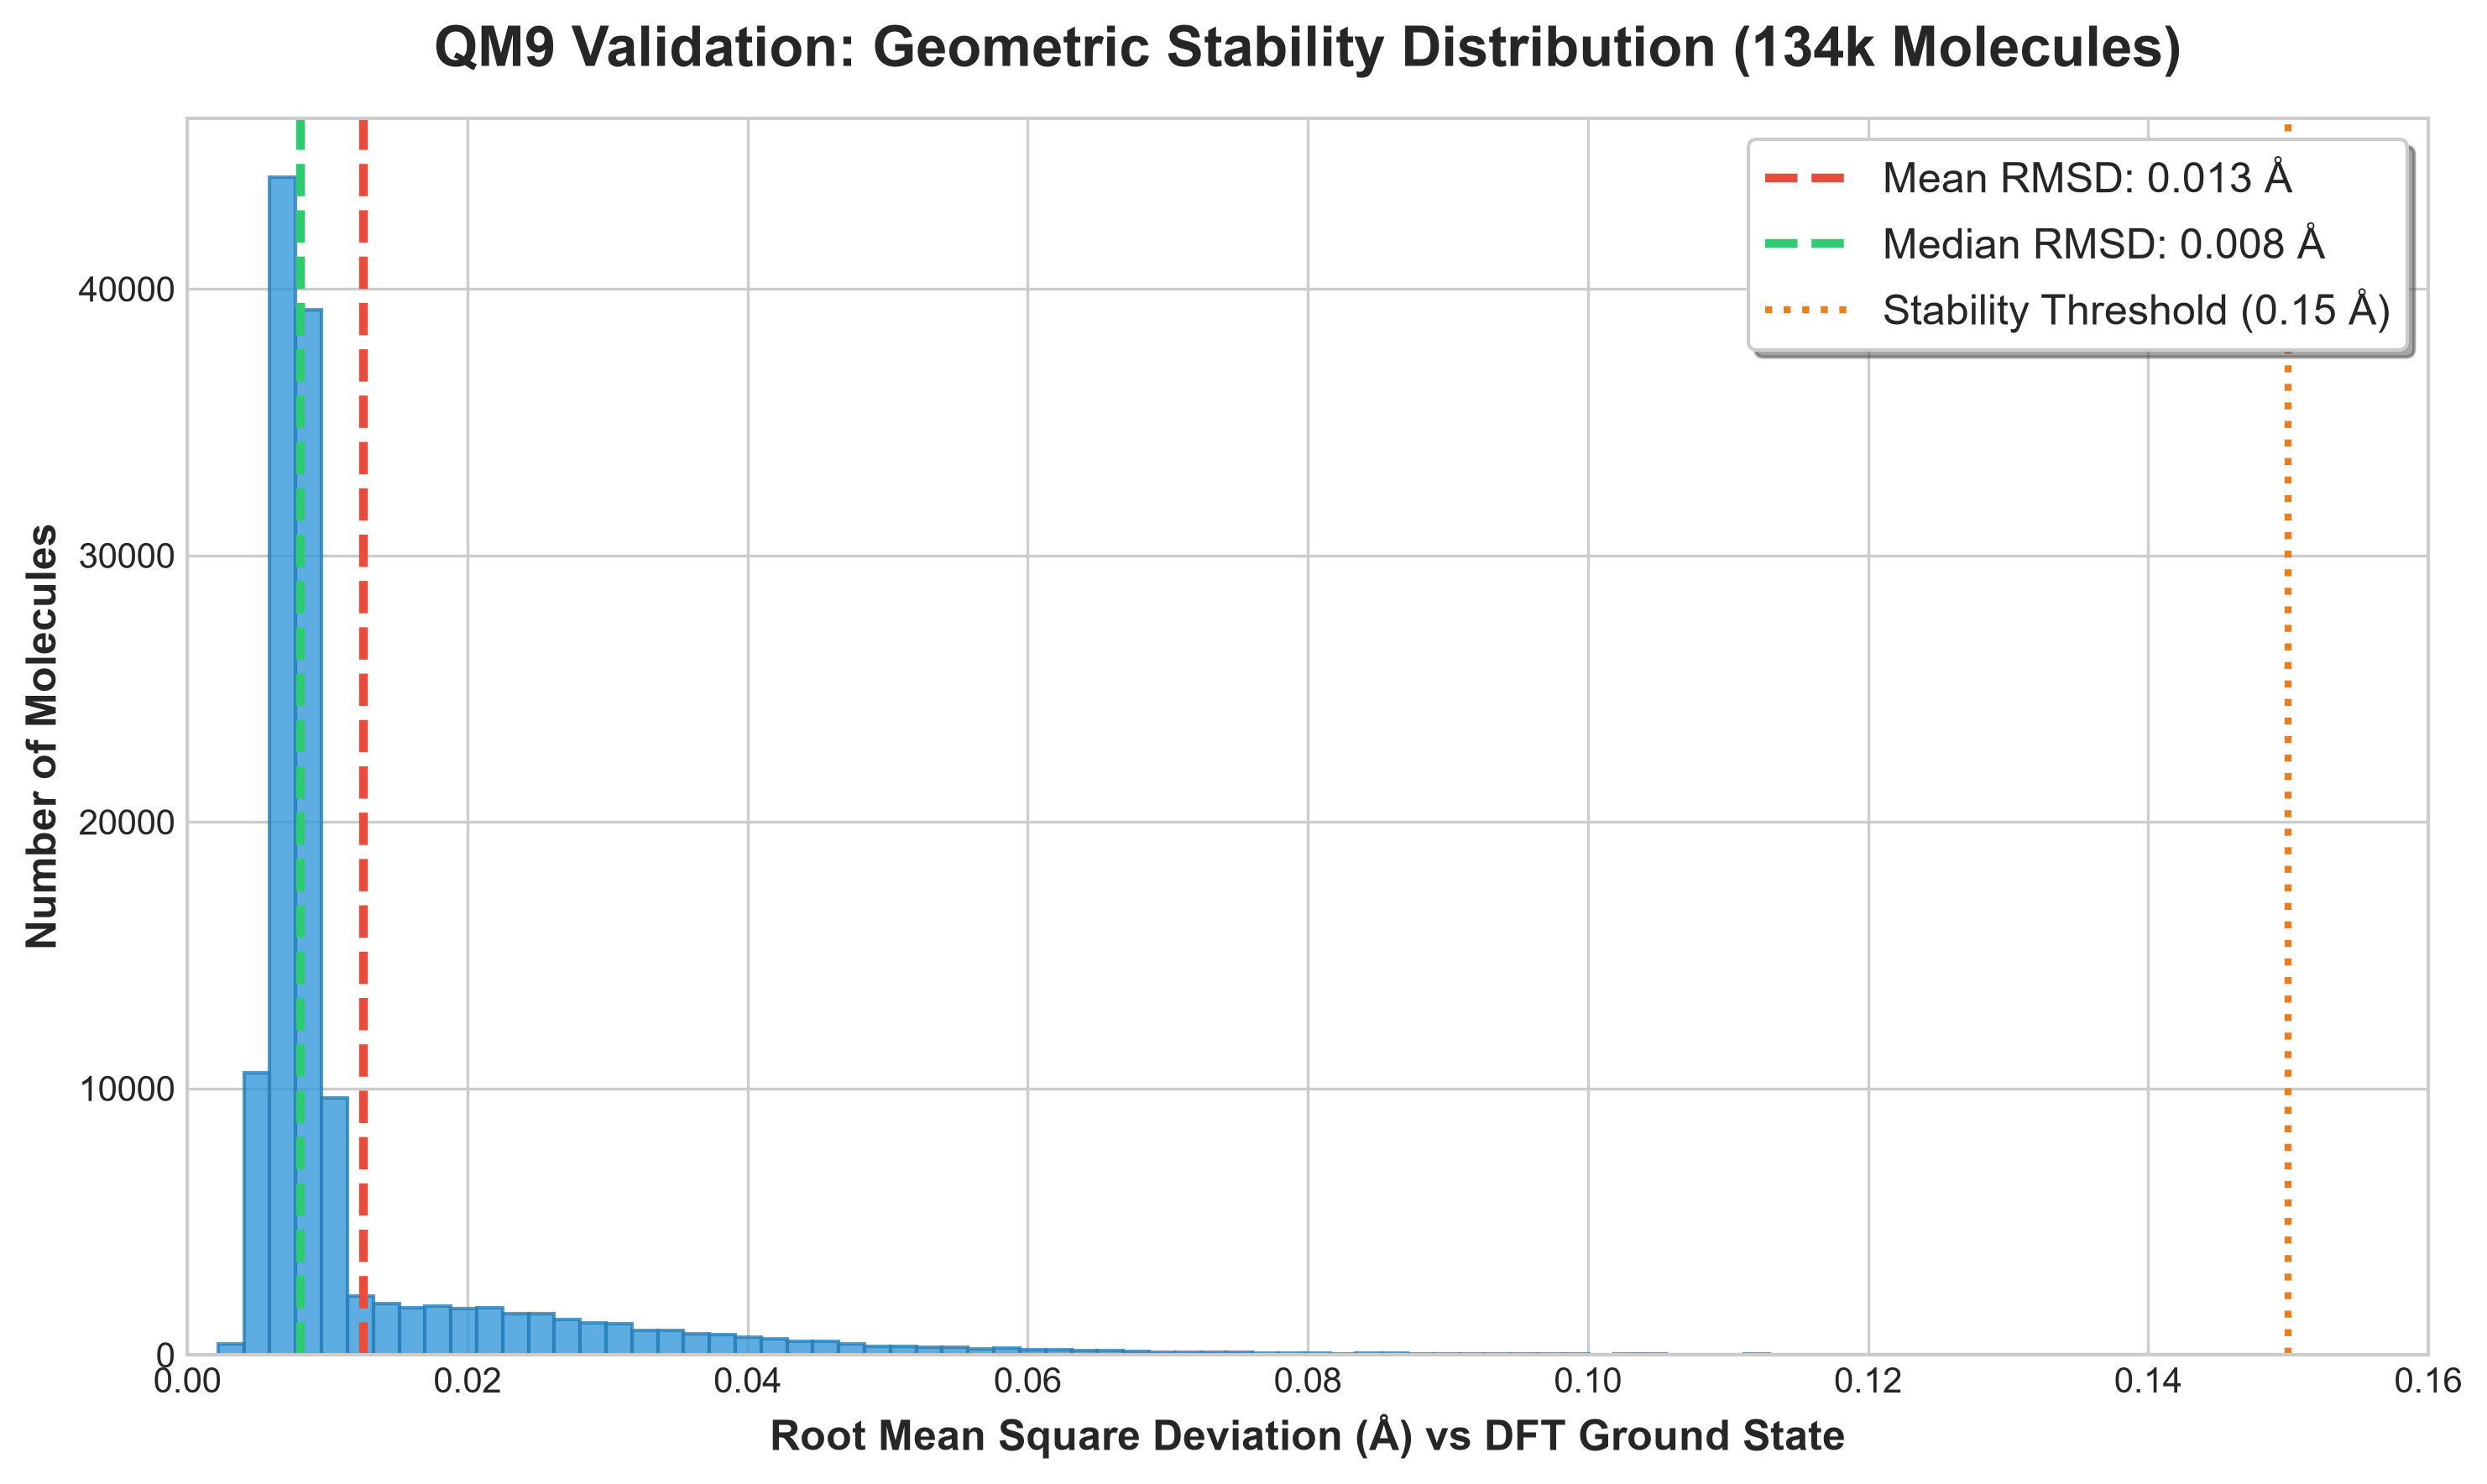
\includegraphics[keepaspectratio,alt={QM9 Validation: RMSD Distribution}]{./experiments/05_QM9_Validation/qm9_rmsd_histogram.png}}
\caption{QM9 Validation: RMSD Distribution}
\end{figure}

A notable theoretical triumph of this high-throughput test was the
seamless integration of Fluorine (\(Z=9\)). In classical chemistry
models, extreme lone-pair repulsion often demands ad-hoc,
element-specific scaling factors to prevent geometric collapse.
Remarkably, in EVM this extreme chemical nature is reproduced
organically. Without altering the universal phase exclusion constant of
the field medium (\texttt{Excl\ =\ 2.0}), EVM maintains structural
stability by simply accounting for the naturally more compact physical
radius of the Fluorine core (\(R=0.14\)). This confirms that complex
quantum-like repulsion effects can emerge naturally from simple,
universal kinematic rules, scaling robustly across hundreds of thousands
of diverse structures.

\subsubsection{3.8. Computational Scaling
Profile}\label{computational-scaling-profile}

{\def\LTcaptype{none} % do not increment counter
\begin{longtable}[]{@{}
  >{\raggedright\arraybackslash}p{(\linewidth - 6\tabcolsep) * \real{0.2500}}
  >{\raggedright\arraybackslash}p{(\linewidth - 6\tabcolsep) * \real{0.2500}}
  >{\raggedright\arraybackslash}p{(\linewidth - 6\tabcolsep) * \real{0.2500}}
  >{\raggedright\arraybackslash}p{(\linewidth - 6\tabcolsep) * \real{0.2500}}@{}}
\toprule\noalign{}
\begin{minipage}[b]{\linewidth}\raggedright
Method
\end{minipage} & \begin{minipage}[b]{\linewidth}\raggedright
Complexity
\end{minipage} & \begin{minipage}[b]{\linewidth}\raggedright
Hardware Required
\end{minipage} & \begin{minipage}[b]{\linewidth}\raggedright
Estimated Runtime
\end{minipage} \\
\midrule\noalign{}
\endhead
\bottomrule\noalign{}
\endlastfoot
\textbf{Ab-Initio (DFT)} & \(O(N^3)\) & Supercomputer Cluster &
\textbf{Months} (Practically impossible) \\
\textbf{EVM} & \(O(N^2)\) & 1x Standard Consumer GPU & \textbf{Minutes}
(Real-time dynamics) \\
\end{longtable}
}

\begin{center}\rule{0.5\linewidth}{0.5pt}\end{center}

\subsection{4. Discussion and Future
Work}\label{discussion-and-future-work}

\subsubsection{4.1. Electron Localization and Polar
Centroids}\label{electron-localization-and-polar-centroids}

A unique aspect of explicit-electron classical models is that we can
trace the coordinates of individual electrons. During our advanced
audits, we measured the centroid of the shared electron cloud in
covalent bonds:

\[
r_{ratio} = \frac{d(e, \text{Heavy})}{d(e, H)}
\]

In standard quantum mechanics, electronegative atoms like Oxygen draw
the bonding electrons closer, making the bond polar. In EVM, the massive
classical Coulomb attraction of the Heavy nuclei (\(Z=6, 7, 8\))
overwhelms the isolated Hydrogen (\(Z=1\)).

As a result, the valence bonding electrons are physically pulled
extremely close to the heavy cores and reside far from the Hydrogen
nucleus (\(d(e, \text{Heavy}) \approx 0.15\) Å
vs.~\(d(e, H) \approx 0.90\) Å), yielding an average ratio
\(r_{ratio} \approx 0.15 - 0.30\). This indicates an ``extreme
polarity'' in classical point-charge dynamics where the proton is left
highly exposed. While this is a structural artifact of classical
point-charge limitations, the overall molecular geometries remain highly
stable because the empirical parameters (\(R_C > R_N > R_O\))
geometrically compensate for the charge shift.

\subsubsection{4.2. Kinematic Limitations and Future Theoretical
Extensions}\label{kinematic-limitations-and-future-theoretical-extensions}

In the current foundational version (EVM 4.0), the kinematic resistance
of Larmor precession (the RAKTS Kinematic Barrier) is simplified to
static phase domains. While sufficient for structural equilibrium and
non-covalent interactions, the lack of real-time dynamic spin precession
(Vector Snap) limits the engine's ability to organically resolve complex
transition states during reactive collisions. Full 3D time-dependent
field kinematics represents the theoretical frontier for future
computational physics engines.

\begin{center}\rule{0.5\linewidth}{0.5pt}\end{center}

\subsection{5. Code Availability \&
Reproducibility}\label{code-availability-reproducibility}

The EVM engine, alongside all tensor configurations and Python scripts
required to reproduce the geometries and benchmarks presented in this
paper, are completely open-source. The repository is publicly available
at: https://github.com/rt20bg/Anastasov\_Theory

\textbf{To reproduce the QM9 benchmarks:} 1. Clone the repository. 2.
Create a virtual environment and install the dependencies:
\texttt{pip\ install\ -r\ requirements.txt}. 3. Download the
\texttt{gdb9.sdf} dataset (see \texttt{data/README.md} for instructions
and links). 4. Run
\texttt{python\ experiments/05\_QM9\_Validation/validate\_qm9.py}.

\begin{center}\rule{0.5\linewidth}{0.5pt}\end{center}

\subsection{References}\label{references}

{[}1{]} Anastasov, I. (2026). \emph{The Rapid Alignment Kinematic Theory
of Spin (RAKTS)}. Zenodo. https://zenodo.org/records/20936532 \textbar{}
https://rt20bg.github.io/Anastasov\_Theory/

\end{document}
